\documentclass[aspectratio=169]{beamer}
%\documentclass[draft]{beamer}

\pdfpageattr {/Group << /S /Transparency /I true /CS /DeviceRGB>>}

\usepackage{tikz}
\usepackage{graphicx}
\usepackage{animate}
\usepackage{media9}
\usepackage{array}

\usetheme{CambridgeUS}
\usecolortheme{dove}

\setbeamersize{text margin left=0cm,text margin right=0cm}
\setbeamerfont{frametitle}{size=\small}
\setbeamertemplate{footline}{}
\setbeamertemplate{navigation symbols}{}

\definecolor{grayed}{gray}{0.85}
\definecolor{lightred}{rgb}{0.8,0.2,0.1}

\begin{document}

\begin{frame}

  \vspace{.3cm}
  \begin{columns}[onlytextwidth,T]
    
    \onslide<1-4>
    \begin{column}{0.3\textwidth}
      \centering
      \only<4>{\textbf}E\only<4>{\color{lightgray}}XPOSURE\\[.2cm]
      \only<1-3>{\begin{tikzpicture}
      \node[opacity=1]{\includegraphics[scale=0.4]{/home/casey/Research/Graphics_Repo/exposure.png}};
      \end{tikzpicture}
      }
      \only<4>{\begin{tikzpicture}
      \node[opacity=.2]{\includegraphics[scale=0.4]{/home/casey/Research/Graphics_Repo/exposure.png}};
      \end{tikzpicture}
      }
    \end{column}
    
    \onslide<2-4>
    \begin{column}{0.01\textwidth}
      \centering
      $\times$
    \end{column}
    
    \onslide<2-4>    
    \begin{column}{0.32\textwidth}
      \centering
      \only<4>{\textbf}H\only<4>{\color{lightgray}}AZARD\\[.2cm]
      \only<2-3>{\begin{tikzpicture}
      \node[opacity=1]{\includegraphics[scale=0.4]{/home/casey/Research/Graphics_Repo/hazard.png}};
      \end{tikzpicture}
      }
      \only<4>{\begin{tikzpicture}
      \node[opacity=.2]{\includegraphics[scale=0.4]{/home/casey/Research/Graphics_Repo/hazard.png}};
      \end{tikzpicture}
      }
    \end{column}
    
    \onslide<3-4>    
    \begin{column}{0.01\textwidth}
      \centering
      $=$
    \end{column}
    
    \onslide<3-4>    
    \begin{column}{0.3\textwidth}
      \centering
      \only<4>{\textbf}R\only<4>{\color{lightgray}}ISK\\[.2cm]
      \only<3>{\begin{tikzpicture}
      \node[opacity=1]{\includegraphics[scale=0.4]{/home/casey/Research/Graphics_Repo/risk.png}};
      \end{tikzpicture}
      }
      \only<4>{\begin{tikzpicture}
      \node[opacity=.2]{\includegraphics[scale=0.4]{/home/casey/Research/Graphics_Repo/risk.png}};
      \end{tikzpicture}
      }
    \end{column}

​  \end{columns}

    \hspace{0cm}
    \centering
    \only<4>{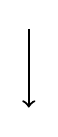
\begin{tikzpicture}
      \coordinate (A);
      \node[below of=A,coordinate] (B) {};
      \draw[->, thick] (A) -- (B);
    \end{tikzpicture}}

    \vspace{0cm}    
    \hspace{.7cm}
    \begin{minipage}[T]{.85\textwidth}
      \centering
      \only<4>{
\begin{tikzpicture}
      \node[fill=grayed,rounded corners=2pt] {
      \large Generalised Linear Model};
      \end{tikzpicture}}
    \end{minipage}

    \vspace{-.5cm} 
    \onslide<5-7>
    \begin{table}[h]
    \begin{tabular}{>{\centering\arraybackslash}m{5.25cm}>{\centering\arraybackslash}m{.4cm}>{\centering\arraybackslash}m{2.2cm}>{\centering\arraybackslash}m{.4cm}>{\centering\arraybackslash}m{2cm}>{\centering\arraybackslash}m{.4cm}>{\centering\arraybackslash}m{2cm}}
    RISK     & $=$     & EXPOSURE     & $\times$     & \multicolumn{3}{c}{HAZARD}\\
               \includegraphics[scale=0.15]{/home/casey/Research/Graphics_Repo/risk.png} &  & \includegraphics[scale=0.15]{/home/casey/Research/Graphics_Repo/exposure.png} &  & \multicolumn{3}{c}{\includegraphics[scale=0.15]{/home/casey/Research/Graphics_Repo/hazard.png}}\\
    \multicolumn{1}{l}{}  & \multicolumn{1}{l}{} & \only<2-3>{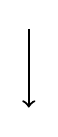
\begin{tikzpicture}
      \coordinate (A);
      \node[below of=A,coordinate] (B) {};
      \draw[->, thick, opacity=1] (A) -- (B);
    \end{tikzpicture}
    }  & \multicolumn{1}{l}{} & \multicolumn{3}{c}{ \only<2-3>{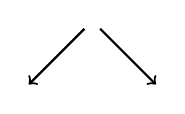
\begin{tikzpicture}
      \coordinate (A);
      \node[below left of=A,coordinate] (B) {};
      \node[below right of=A,coordinate] (C) {};
      \draw[->, thick, opacity=1] ([xshift=-.7cm]A.center) -- ([xshift=-.7cm]B.center);
      \draw[->, thick, opacity=1] ([xshift=-.5cm]A.center) -- ([xshift=-.5cm]C.center);
    \end{tikzpicture}
    }}\\
  \only<6-7>{\scriptsize{Collision}     & $\approx$     & \includegraphics[scale=0.25]{/home/casey/Research/Graphics_Repo/pred_brt.png} & $\times$ & \includegraphics[scale=0.07]{/home/casey/Research/Graphics_Repo/traffic_vol2.png} & $\times$ & \includegraphics[scale=0.07]{/home/casey/Research/Graphics_Repo/traffic_spd2.png}\\
        &        & \tiny{Kangaroo Presence} & & \tiny{Vehicle Volume} & & \tiny{Vehicle Speed}} 
    \end{tabular}
    \end{table}

    \onslide<7>
    \vspace{-.25cm} 
    \begin{minipage}[T]{1\textwidth}
      \centering
      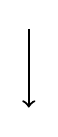
\begin{tikzpicture}
      \coordinate (A);
      \node[below of=A,coordinate] (B) {};
      \draw[->, thick, opacity=1] (A) -- (B);
      \end{tikzpicture}

      
\begin{tikzpicture}
      \definecolor{grayed}{gray}{0.85}	  
	  \node[fill=grayed,rounded corners=2pt] {
      \large Logistic Regression Model};
      \end{tikzpicture}
  
    \end{minipage}
    
    \onslide<8>
    \vspace{-.25cm} 
    \begin{minipage}[T]{1\textwidth}
      \centering
      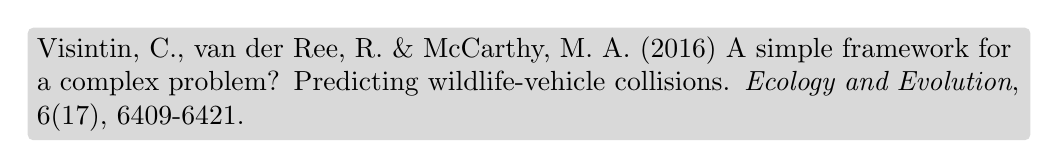
\begin{tikzpicture}
      \definecolor{grayed}{gray}{0.85}
      \node[fill=grayed,rounded corners=2pt, text width=12.5cm] {
      Visintin, C., van der Ree, R. \& McCarthy, M. A. (2016) A simple framework for a complex problem? Predicting wildlife-vehicle collisions.  \textit{Ecology and Evolution}, 6(17), 6409-6421.};
      \end{tikzpicture}
    \end{minipage}

\end{frame}

\end{document}